\documentclass[a4paper,11pt,dvipdfmx]{jsarticle}


% 数式
\usepackage{amsmath,amsfonts}
\usepackage{bm}

% 画像
\usepackage[dvipdfmx]{graphicx}
\usepackage{framed}

% 図形
\usepackage{tikz}
\usetikzlibrary{shapes.geometric}
\usetikzlibrary {shapes.misc}

% ソースコード
\usepackage{listings,jlisting,color}
\lstset{
basicstyle={\ttfamily},
identifierstyle={\small},
commentstyle={\smallitshape},
keywordstyle={\small\bfseries},
ndkeywordstyle={\small},
stringstyle={\small\ttfamily},
frame={tb},
breaklines=true,
columns=[l]{fullflexible},
numbers=left,
xrightmargin=0zw,
xleftmargin=3zw,
numberstyle={\scriptsize},
stepnumber=1,
numbersep=1zw,
lineskip=-0.5ex
}
\renewcommand{\lstlistingname}{ソースコード}


\begin{document}
\definecolor{shadecolor}{gray}{0.70}

\title{数値計算 Class-8 演習}
\author{21T2166D 渡辺大樹}
\date{\today}
\maketitle

\section{演習内容}
Class-8でも引き続き、いくつかの$xy$平面上のデータからそのデータをすべて通るなめらかな曲線を描くための手法、
最小二乗法についてコードを実装し、実際に動かしていく。

最小二乗法はよく用いられる、データから関数を見つけ出す手法で、
大雑把に言えばデータ点と予測される関数の$y$座標の値の誤差を二乗し、それが最小になる関数を探す手法である。

まず、データ点から予測される関数が単一の一次方程式$y=ax+b$であるときを考える。
データ点はそれぞれ$(x_i,y_i)\quad (i=0,1,\cdots,n)$である。
このときのデータと予測される関数との誤差$E_i$は
\begin{equation}
    E_i = ax_i+b-y_i
\end{equation}
で表される。

これを二乗してすべてのデータ点で足し合わせることで二乗誤差$E$を得る。
\begin{align}
    E &= \sum_{i=0}^{n}(E_i)^2 \notag \\
      &= \sum_{i=0}^{n}(ax_i+b-y_i)^2
\end{align}

これを最小にする$a,b$を決めたいので$a,b$それぞれで(2)の式を偏微分することで
\begin{align}
    \frac{\partial E}{\partial a} &= \frac{\partial \sum_{i=0}^{n}(ax_i+b-y_i)^2}{\partial a} \notag \\
                                  &= \sum_{i=0}^{n}2x_i(ax_i+b-y_i) \\
    \frac{\partial E}{\partial b} &= \frac{\partial \sum_{i=0}^{n}(ax_i+b-y_i)^2}{\partial b} \notag \\
                                  &= \sum_{i=0}^{n}2(ax_i+b-y_i) 
\end{align}
の(3),(4)の二式が得られる。

この二式イコール0を連立方程式として解けば求めたい$a,b$の係数を得られる。

これを拡張し、一般化すれば任意の関数の一次結合をした関数で誤差の二乗が最小の関数を得ることができる。

詳細は省略するが、任意の適当な$n$個の関数を一次の係数$a_i \quad(i=1,2,\cdots,n)$で一次結合し、
与えられた$n$個のデータ点を代入した連立方程式に関して、
二乗誤差の足し合わせ$E$を$a_i \quad(i=1,2,\cdots,n)$で偏微分することによって得られる連立方程式を掃き出し法
などを用いて解くことで一次の係数$a_i \quad(i=1,2,\cdots,n)$を求めることができる。

以上の最小二乗法によるなめらかな関数を求めるアルゴリズムは以下のソースコード\ref{minjijo}で実装される。
\lstinputlisting[caption=minjijo.c, label=minjijo]{C:/Program_Code/NumMeth/Class8/minjijo.c}

コード上では77行目まででデータの関係関数の入力と、実際のデータの入力を行っている。

83行目からは二乗誤差を偏微分し、足し合わせることで出てくる$\textbf{a}$の係数行列$A^TA$を計算し、
それをもとに97行目からガウスジョルダン法を用いて連立方程式を解いている。

解けた解はd[1],d[2]として出力され、グラフを書くためにデータの$x$の最大値最小値を50分割した関数の値を
出力できるようにしている。

\section{演習結果}
演習として以下のデータ表から最小二乗法でなめらかな関数を出力する。
\begin{center}
    \begin{tabular}[h]{|c|c|c|c|c|c|c|c|c|} \hline
         $x$  & 0.01 & 0.1 & 0.5 & 1.0 & 2.0 & 4.0 & 8.0 & 10.0 \\ \hline
         $y$  & 218  & 26  &  8  &  4  &  1  &  8  &  31 &  230 \\ \hline
    \end{tabular}
\end{center}

Excelなどでプロットするとわかるがこれは関係関数として$f(x)=\frac{1}{x},\quad g(x)=e^x$と定めることができる。

実際にこの条件で入力すると
\begin{shaded}
    \noindent
    \centering
    a = d[1] = 2.185093\\
    b = d[2] = 0.010431
\end{shaded}
のような出力を得ることができる。

Pythonを用いてデータ点とこの係数で関係関数を結合した関数$\frac{2.185093}{x}+0.010431e^x$をプロットすると
以下図\ref{fig:1}のようなグラフを得られる。

\begin{figure}[h] 
    \centering
    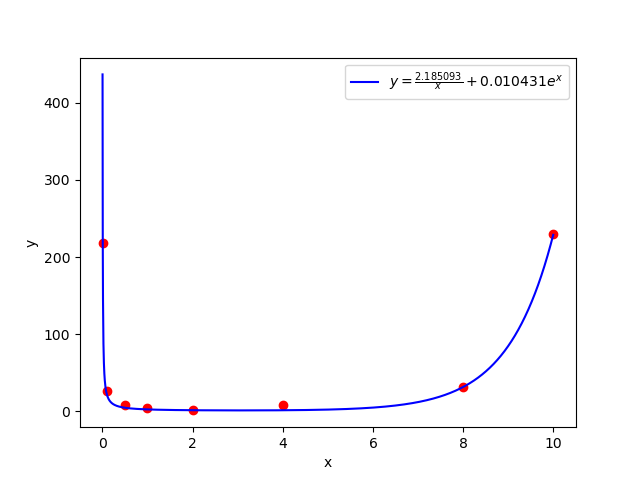
\includegraphics[width=80mm]{./plot.png}
    \caption{ソースコード\ref{minjijo}で得られた関数とデータ点のプロット}
    \label{fig:1}
\end{figure}

この図\ref{fig:1}より誤差の少ない関数を取得できていることが確認できる。

教科書の演習問題も解いていく。

(a) 

以下の表を$y=ax+b$で解く。
\begin{center}
    \begin{tabular}[h]{|c|c|c|c|c|c|} \hline
         $x$  & 1.0 & 2.0 & 3.0 & 4.0 & 5.0 \\ \hline
         $y$  & 2.0 & 2.5 & 2.9 & 3.5 & 4.4 \\ \hline
    \end{tabular}
\end{center}

結果はこのように得られた。

\begin{shaded}
    \noindent
    \centering
    a = d[1] = 0.580000\\
    b = d[2] = 1.320000
\end{shaded}

答えと一致する値となった。

(b) 

以下の表を$y=ax+\frac{b}{x}$で解く。
\begin{center}
    \begin{tabular}[h]{|c|c|c|c|c|c|c|c|} \hline
         $x$  &  0.2 & 0.5 & 1.0 & 2.0 & 4.0 & 8.0 & 10.0 \\ \hline
         $y$  & 12.1 & 4.9 & 2.9 & 2.1 & 2.1 & 3.4 &  4.3 \\ \hline
    \end{tabular}
\end{center}

結果はこのように得られた。

\begin{shaded}
    \noindent
    \centering
    a = d[1] = 0.398093\\
    b = d[2] = 2.401050
\end{shaded}

答えと一致する値となった。

(c) 

以下の表を$y=ax+b$で解く。
\begin{center}
    \begin{tabular}[h]{|c|c|c|c|c|c|} \hline
         $x$  & 1.0 & 1.5 & 2.0 & 3.0 &  5.0 \\ \hline
         $y$  & 2.4 & 4.0 & 6.2 & 9.5 & 17.1 \\ \hline
    \end{tabular}
\end{center}

結果はこのように得られた。

\begin{shaded}
    \noindent
    \centering
    a = d[1] = 3.680000\\
    b = d[2] = -1.360000
\end{shaded}

答えと一致する値となった。

(d) 

以下の表を$y=ax+b$で解く。
\begin{center}
    \begin{tabular}[h]{|c|c|c|c|c|c|c|c|c|c|} \hline
         $x$  & 18 & 28 & 38 & 48 & 58 & 68 & 78 & 88 & 98 \\ \hline
         $y$  & 15.2 & 15.9 & 16.7 & 16.9 & 17.4 & 18.0 & 18.7 & 19.3 & 19.8 \\ \hline
    \end{tabular}
\end{center}

結果はこのように得られた。

\begin{shaded}
    \noindent
    \centering
    a = d[1] = 0.056167\\
    b = d[2] = 14.286778
\end{shaded}

答えと一致する値となった


\end{document}